\section{Software testing}
\label{sec:related:testing}

Software testing is the process of executing a program or system
with the intent of finding errors \cite{Myers:1979:AST:539883}.
However, testing shows the presence, not the absence of bugs as
Edsger Wybe Dijkstra used to say.

Testing is achieved by analyzing a software to detect the
differences between existing and required conditions (that is,
bugs) and to evaluate the features of this software. As Meyers
said, testing is used to find faults, but it is also useful to
provide confidence of reliability, correctness, and absence of
particular faults on software we develop. This does not mean that
the software is completely free of defects. Rather, it must be
good enough for its intended use.
Testing is a verification and validation process
\cite{wallace1989software}. I use to (informally) explain both
terms with the following questions \cite{Boehm1979}:

\begin{itemize}
\item \textbf{Validation:} are we building the right software?
\item \textbf{Verification:} are we building the software right?
\end{itemize}

In other words, formal verification is the act of proving or
disproving the correctness of intended algorithms underlying a
system with respect to a certain formal specification or
property, using formal methods of mathematics. Model checking,
runtime verification, theorem proving, static analysis and
simulation are all verification methods.

Validation is testing as the act of revealing bugs. That is what
most people think testing is, and also the meaning we give to the
word "testing" in the sequel of this thesis. Testing involves a
(software) \textit{system under test} (SUT). \textit{Test inputs}
are sent on a system under test, which leads to \textit{test
outputs}. We then have to determine whether these outputs are
correct. A \textit{test case} (TC) is compound of \textit{test
data}, i.e.  inputs which have been devised to test the system,
an expected behavior, and an expected output. We call
\textit{test suite} (TS) a set of test cases. We rely on a
\textit{tester} to determine whether a test has \textit{passed}
or \textit{failed}. Those two words are known as
\textit{verdicts}.

In the following section, we introduce the software testing
realm. We focus on Model-based Testing, presented in Section
\ref{sec:related:testing:mbt} along with some definitions used
in the rest of this thesis.

\subsection{Types of testing}

\begin{figure}[ht]
    \begin{center}
    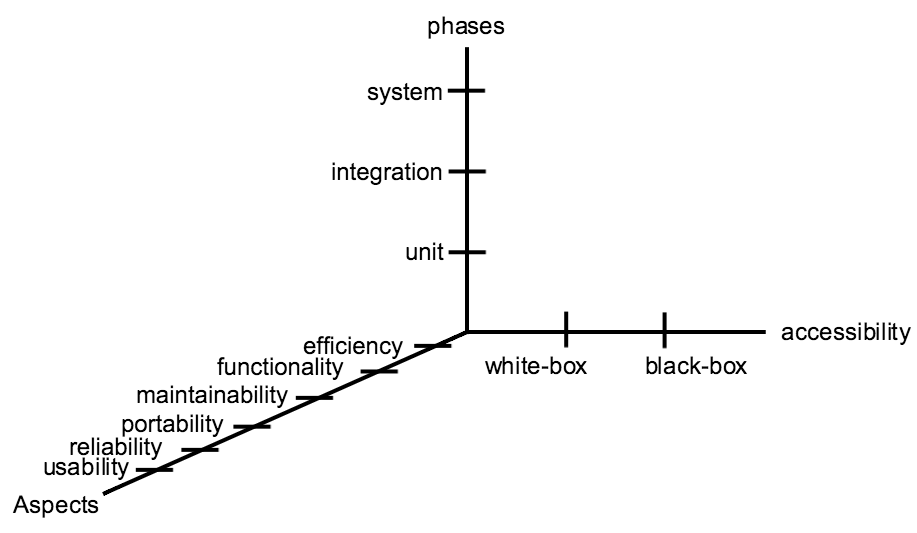
\includegraphics[width=1.0\linewidth]{figures/sorts-of-testing.png}
    \end{center}

    \caption{Sorts of testing}
\end{figure}

Nowadays, software testing, if not always applied, is well-known
in the Industry. It is considered a good practice and many
techniques and tools have been developed over the last 10 years.
Most of them are different in nature and have different purposes.
There are a lot of new terms that all end with "Testing" such as:
Unit Testing, Integration Testing, Functional Testing, System
Testing, Stress Testing, Performance Testing, Usability Testing,
Acceptance Testing, Regression Testing, Beta Testing, and so on.

ISO 9126 \cite{iso9126}, replaced by ISO/IEC 25010:2011
\cite{10951538}, provides six characteristics of quality that can
be used to sort these testing techniques into six testing types:

\begin{itemize}
\item efficiency testing,
\item functionality testing,
\item maintainability testing,
\item portability testing,
\item reliability testing,
\item usability testing.
\end{itemize}

However, this classification can not be generally accepted as
single or complete. In \cite{4425813}, authors suggested to
classify the different techniques based on the target of the
test (sometimes we refer to this classification as level of
detail):

\begin{itemize}
\item \textbf{Unit Testing:} units (e.g., functions, methods,
modules) of the system are tested in isolation. Typically this
testing type implies access to the source code being tested,

\item \textbf{Integration Testing:} interactions between software
components are tested. This testing type is a continuous task,
hence the \textit{continous integration} (CI) practice,

\item \textbf{System Testing:} the whole system is taken into
consideration. This testing type is appropriate for validating
not-only-functional requirements, such as security, performance
(speed), accuracy, and reliability (fault tolerence).
\end{itemize}

These requirements are sometimes seen as \textit{objectives} of
testing, leading to even more different testing types as listed
before. There are also different approaches to perform testing,
depending on the information available to construct the test
cases:

\begin{itemize}
\item \textbf{white-box:} a method that tests the internal
structure of a SUT. It is usually done at the unit level,

\item \textbf{black-box:} a method that tests the functionalities
of a SUT without knowing its internal structure.  It is also
known as functional testing,

\item \textbf{grey-box:} the combination of white-box testing and
black-box testing. One has access to the relevant internal parts
of a SUT.
\end{itemize}

Because testing cannot guarantee the absence of faults, a
challenge is to select subset of test cases from all possible
test cases with a high chance of detecting most faults. A lot of
research on \textit{test selection} (or strategies) has been
done, and there are numerous existing methods for both black-box
and white-box approaches.

\paragraph{Black-box strategies} Combinatorial Testing (also
known as Pairwise) \cite{Tai98atest} is based on the observation
that most faults are caused by interactions of at most two
factors. Here we test all the possible discrete combinations of
the parameters involved.  Because we cannot test all the possible
input domain values for practical reasons, Equivalence
Partitioning \cite{Huang13} is a technique that divides the test
input data into a range of values, and selects one input value
from each range. Similarly, Boundary Value Analysis
\cite{Ramachandran:2003:TSC:942796.943301} is used to find the
etechniquesrrors at boundaries of input domain rather than finding those
errors in the center of input. We can also mention Functional
Coverage (also known as Inductive Testing)
\cite{Walkinshaw:2010:IFC:1928028.1928038} where a test set is
good enough when it achieves a given level of coverage.

\paragraph{White-box strategies} Fuzz Testing also known as
Random Testing
\cite{Duran:1981:RRT:800078.802530,Godefroid08automatedwhitebox}
is a method that applies random mutations to well-formed inputs
of a program, and test the resulting values. Such a technique can
also be applied using a black-box approach though, e.g.,
\cite{5387827}.  Statistical Testing
\cite{Walton:1995:STS:210453.210458} is a technique where test
data is generated by sampling from a probability distribution
chosen so that each element of the software's structure is
exercised with a high probability. We can also mention all
techniques related to the code structure, such as Statement
Testing, Path Testing, Branch Testing, Condition Testing,
Multiple Condition (MC) Testing, and Loop Testing.  Another
technique acts on the source code by mutating it, i.e.  seeding
the implementation with a fault by applying a mutation operator,
and then determining whether testing identifies this fault. This
is known as Mutation Testing \cite{1702444}.

While the Industry created many different testing tools (often
originating from Academia), they mostly perform testing by hand.
Researchers in software testing have worked for decades on
automatic test generation. Automatic testing is, for instance,
one way to automate white-box approaches, but there are many
other techniques. On the contrary, Model-based Testing (MbT) is
one research area that tries to automate black-box approaches.
In this thesis, we are interested in making production systems
more reliable by means of Model-based Testing.

\subsection{Model-based Testing}
\label{sec:related:testing:mbt}

\begin{figure}[ht]
    \begin{center}
    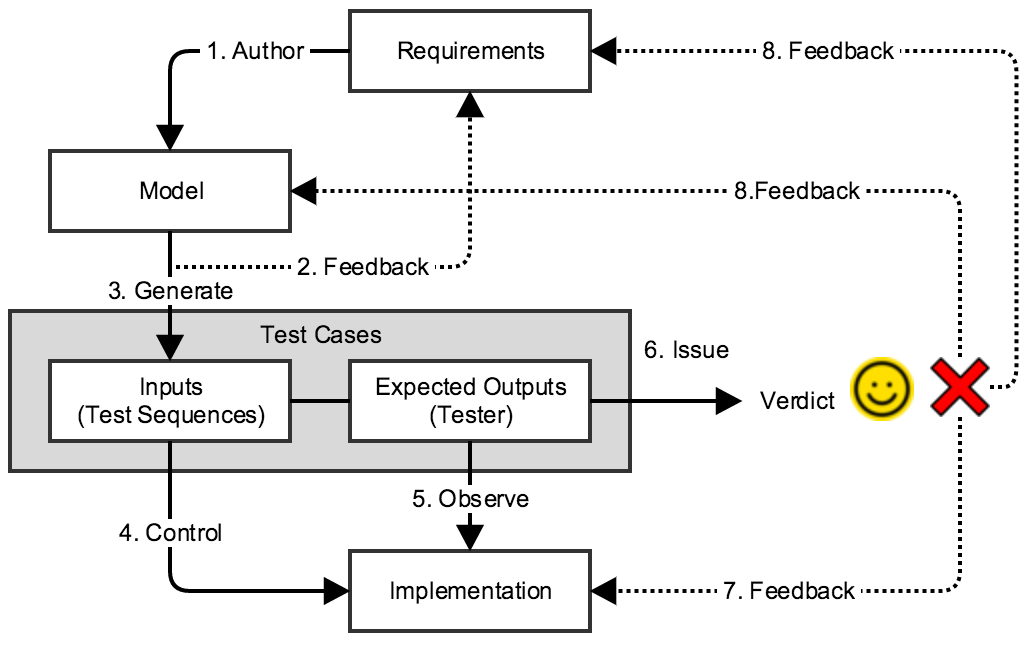
\includegraphics[width=1.0\linewidth]{figures/mbt.png}
    \end{center}

    \caption{A simplified diagram showing how MBT works}
    \label{fig:mbt}
\end{figure}

\textit{Model-based Testing} (MbT) is application of Model-based
design for designing and optionally also executing artifacts to
perform software testing \cite{Jorgensen:1995:STC:526521}.
Models can be used to represent the desired behavior of an SUT,
or to represent testing strategies and a test environement.
Model-based Testing can be summarized as a three-step process,
which is extended in Figure \ref{fig:mbt}:

\begin{enumerate}
\item Formally modelling the requirements (specification),

\item Generating test cases from the model,

\item Running these test cases against an actual SUT and
evaluating the results.
\end{enumerate}

\subsubsection{What is a model?}
\label{sec:related:testing:model}

Generally speaking, a model is a representation of a thing that
allows for investigation of its properties, and most of the time,
a model hides the complexity of the item it represents. In the
software engineering field, models help describe software systems
in order to: (i) ease the process of studying them, (ii) leverage
them to build tools or generate documentation, (iii) reveal
defects (validation or verification).

Such models usually describe the behaviors of the software being
modeled, and can also be known as specifications, helping
understand and predict its behavior. There are numero models for
modeling software systems, and each describes different aspects
of software behavior. For example, control flow, data flow, and
program dependency graphs express how the implementation behaves
by representing its source code structure. It is worth mentioning
that a model does not have to completely describe it to be
effective.

We can classify models that can be employed for testing into two
categories:

\begin{itemize}
\item \textbf{Behavior/Control oriented:} Finite Automata (like
Finite State Machines, Symbolic Transition Systems, and Labelled
Transition Systems) are well-known in software testing. They are
very generic and flexible, and are a good fit when it comes to
model software systems. For real-time and/or safety-critical
systems, we often rely on Synchronous Languages such as Lustre
\cite{lustre:ieee} and SCADE
\cite{LeSergent:2011:SCF:2188575.2188578}. We can also mention
Petri Nets,

\item \textbf{Data oriented (pre/post):} often using annotation
languages originating from the \textit{Design-By-Contract}
paradigm \cite{Meyer:1992:ADC:618974.619797}. These languages
make it possible to express formal properties (invariants,
pre/post-conditions) that directly annotate program entities
(such as classes, methods, attributes) in the source code. Many
annotation languages exist, such as the Java Modeling Language
\cite{jml}, Spec\# \cite{117852}, the Object Constraint Language
\cite{Warmer:1998:OCL:291202}, the B-Method
\cite{Lano:1996:BLM:525749}, and Praspel
\cite{Enderlin:2011:PSL:2075545.2075551}.
\end{itemize}

In \cite{Sommerville:1997:REG:549198}, Sommerville and Sawyer
give some guidelines for choosing a model for software
requirements. The choice of a model depends on many factors, such
as aspects of the system under test or the testing goal.  Below
we introduce a few definitions of formal models that we use in
this thesis. We mainly work with behavior-oriented models that
are finite automata since they are particularly suitable for
modeling both web applications and production systems behaviors.

\paragraph{Symbolic Transition Systems}
\label{sec:definitions:sts}

The \textit{Symbolic Transition System} (STS) is known as a very
general and powerful model for describing several aspects of
event-based systems. The use of symbolic variables helps describe
infinite state machines in a finite manner. This potentially
infinite behaviour is represented by the semantics of a STS,
given in terms of \textit{Labelled Transition System} (LTS). STS
operations and transformations are often given with inference
rules.

We briefly give some definitions related to the STS model below,
but we refer to \cite{FTW05} for a more detailed description.

\begin{definition}[Variable assignment]
We assume that there exist a domain of values denoted $D$ and a
variable set $X$ taking values in $D$. The assignment of
variables in $Y \subseteq X$ to elements of $D$ is denoted with a
mapping $\alpha: Y \rightarrow D$. $\alpha(x)$ denotes the
assignment of the variable $x$ to a value in $D$.

We denote $D_Y$ the assignment set over $Y$. We also denote
$id_Y$ the identity assignment over $Y$. Finally, $v_\emptyset$
is the empty assignment.
\end{definition}

\begin{definition}[Symbolic Transition System]
	A Symbolic Transition System (STS) consists of locations and
    transitions between locations. It is defined as a tuple $<
    L,l_0,V,V_0,I,\Lambda,$ $\rightarrow>$, where:

	\begin{itemize}
        \item STSs do not have \textbf{states but locations}
        (a.k.a. symbolic states), and $L$ is the finite location
        set, with $l_0$ being the initial one,

        \item $V$ is the finite set of internal variables, while
        $I$ is the finite set of parameters. The internal
        variables are initialised with the condition $V_0$ on
        $V$,

        \item $\Lambda$ is the finite set of symbolic actions
        $a(p)$ ($a$ being a symbol), with $p=(p_1,\dots ,p_k)$ a
        finite set of parameters in $I^{k} (k \in \mathbb{N})$,

        \item $\rightarrow$ is the
        finite set of symbolic transitions. A symbolic transition
        $t = (l_i,l_j,a(p),G,\\A)$,
        from the location $l_i \in L$ to $l_j \in L$, also
        denoted $l_i \xrightarrow{a(p),G,A} l_j$, is labelled by:

		\begin{itemize}
            \item an action $a(p) \in \Lambda$,

            \item a guard $G$ over $(p \cup V)$, which
            restricts the firing of the transition. We consider
            guards written as conjunctions of equalities:
            $\displaystyle \bigwedge_{x \in I \cup V} (x == val)$,

            \item an assignment $A$ which defines the evolution
            of the proper variables, $A_x$ being the function in
            $A$ defining the evolution of the variable $x \in V$.
		\end{itemize}
	\end{itemize}

	\label{def:sts}
\end{definition}

We also denote $Proj_{x}(G)$ the projection of the guard $G$ over
the variable $x \in I \cup V$, which extracts the equality
$(x==val)$ from $G$. For example, given the guard $G_1 = [nsys==1
\wedge nsec==8 \wedge point==1 \wedge pid==1]$, $Proj_{nsys}(G_1)
= (nsys==1)$.

For readability purpose, if $A$ is the identity function $id_V$,
we denote a transition with $l_i \xrightarrow{a(p),G} l_j$. We
also use the generalised transition relation $\Rightarrow$ to
represent STS paths: $l \xRightarrow{(a_1,G_1,A_1)\dots
(a_n,G_n,A_n)} l' =_{def} \exists l_0\dots l_n, l=l_0
\xrightarrow{a_1,G_1,A_1} l_1\dots
l_{n-1}\xrightarrow{a_n,G_n,A_n}l_n=l'$.

\paragraph{Labelled Transition Systems}

A STS is associated with a Labelled Transition System (LTS) to
formulate its semantics. Intuitively, a LTS semantics corresponds
to a valued state machine, without symbolic variables, which is
often infinite: the LTS states are labelled by internal variable
assignments while transitions are labelled by actions combined
with parameter assignments.

\begin{definition}[Labelled Transition System semantics]
    The semantics of a STS $\EuScript{S}=<L,l_0,$ $V,$ $V_0,$
    $I,\Lambda,\rightarrow>$ is the LTS
    $||\EuScript{S}||=<Q,q_0,\sum,\rightarrow>$ where:

	\begin{itemize}

		\item $Q=L \times D_V$ is the set of states,

        \item $q_0=(l_0,V_0)$ is the initial state,

		\item $\sum=\{(a(p),\alpha)  \mid  a(p)\in\Lambda, \alpha \in
		D_p\}$ is the set of valued events,

        \item $\rightarrow$ is the transition relation $Q \times
        \Sigma \times Q$ deduced by the following rule:\\
	\end{itemize}
	\begin{center}
    $\frac{l_1 \xrightarrow{a(p),G,A}l_2,\alpha \in D_p, v \in D_V, v'
        \in D_V, v \cup \alpha \models G, v'=A(v \cup \alpha))}{(l_1,v)
            \xrightarrow{a(p),\alpha} (l_2,v') }$
	\end{center}

	\label{def:semantics}
\end{definition}

This rule can be read as follows: for a STS transition $l_1
\xrightarrow{a(p),G,A}l_2$, we obtain a LTS transition $(l_1,v)$
$\xrightarrow{a(p),\alpha} (l_2,v')$ with $v$ a variable
assignment over the internal variable set, if there exists an
assignment $\alpha$ such that the guard $G$ evaluates to true
with $v \cup \alpha$. Once the transition is executed, the
internal variables are assigned with $v'$ derived from the
assignment $A(v \cup \alpha)$.

In addition, runs and traces, which represent executions and
event sequences, can also be derived from LTS semantics:

\begin{definition}[Runs and traces]
    Given a STS $\EuScript{S}=$ $<L,l_0,V,V_0,I,\Lambda,
	\rightarrow>$, interpreted by its LTS semantics
	$||\EuScript{S}||=<Q,q_0,\sum,\rightarrow>$, a run $q_0
	\alpha_0 \dots \alpha_{n-1} q_n$ is an alternate sequence of states
    and valued actions. $Run(\EuScript{S})=Run(||\EuScript{S}||)$ is
	the set of runs found in $||\EuScript{S}||$.

    It follows that a trace of a run $r$ is defined as the projection
    $proj_{\sum}(r)$ on the actions.

	\label{def:runs-and-traces}
\end{definition}

\paragraph{Input/Output Symbolic Transition Systems}
\label{sec:definitions:iosts}

An Input/Output Symbolic Transition System (IOSTS) is a STS where
the action set is divided into two subsets: one containing the
inputs, beginning by $?$, to express actions expected by the
system, and another containing outputs, beginning by $!$, to
express actions produced by the system.

\begin{definition}[Input/Output Symbolic Transition System]
An Input/Output Symbolic Transition System (IOSTS) $\EuScript{S}$
is a tuple $< L,l0,V,V0,I,\Lambda,\rightarrow>$, where:

\begin{itemize}
\item $L$ is the finite set of locations, $l0$ the initial
location,

\item $V$ is the finite set of internal variables, $I$ is the
finite set of parameters. The internal variables are initialised
with the assignment $V0$ on $V$, which is assumed to be unique,

\item $\Lambda$ is a finite set of symbolic actions $a(p)$, with
$p = (p_1,\dots,p_k)$ a finite list of parameters in $I^k(k \in
\mathbb{N})$. $p$ is assumed unique. $\Lambda= \Lambda^I  \cup
\Lambda^O \cup \{!\delta \}$: $\Lambda^I$ represents the set of
input actions, $\Lambda^O$ the set of output actions, and
$\delta$ the quiescence,

\item $\rightarrow$ is the finite transition set. A transition
$(l_i,l_j,a(p),G,A)$, from the location $l_i \in L$ to $l_j \in
L$, denoted $l_i \xrightarrow{a(p),G,A} l_j$ is labelled by: an
action $a(p) \in \Lambda$, a guard  $G$ over $(p \cup V \cup T(p
\cup V))$ which restricts the firing of the transition. $T(p \cup
V)$ is a set of functions that return boolean values only (a.k.a.
predicates) over $p \cup V$, an assignment function $A$ which
updates internal variables. $A$ is on of the form $(x:=A_x)_{x\in
V}$, where $A_x$ is an expression over $V \cup p \cup T(p \cup
V)$.
\end{itemize}
\end{definition}

\subsubsection{Common terms in MbT}

In this section, we introduce a few common terms defining what
Model-based Testing is, and how it works in general.

Executing a test case on a system yields a set of observations.
Every observation represents a part of the \textit{implementation
model} of the system. The set of all observations made with all
possible test cases represents the complete implementation model
of the system.

\paragraph{Testing hypothesis} For every system there is a
corresponding observational equivalent implementation model:
$\forall \text{ } iut \in IMPS, \exists \text{ } I_{iut} \in
MODS$, where $iut$ is a concrete \textit{implementation under
test} (IUT), $IMPS$ is the universe of implementations, $I_{iut}$
is a model of $iut$, and $MODS$ is the universe of the models of
all IUT.

\paragraph{Implementation relation} To define conformance between
an implementation under test $imp$ and a specification $spec$, we
use the notion of an \textit{implementation relation}: $imp
\subseteq MODS \times SPECS$, with $SPECS$ the set of
specifications. We can find different implementation relations,
e.g., \cite{Bri88,phalippou94}.

\paragraph{Conformance} An implementation $iut$ conforms to a
specification $spec$ if the existing model $I_{iut}$ of $iut$ is
\textit{imp-related} to $spec$. There are many conformance
relations in the literature, which we can organize in three
categories:

\begin{itemize}
\item \textbf{Equivalence relations:} Isomorphism, Bisimulation
\cite{Abdulla06,Fernandez89animplementation}, Trace Equivalence,
Testing Equivalence \cite{Abramsky1987225}, Refusal Equivalence
\cite{DBLP:conf/icalp/Phillips86},

\item \textbf{Preorder relations:} Observation Preorder, Trace
Preorder, Testing Preorder \cite{Beohar2015}, Refusal Preorder,

\item \textbf{Input-Output relations:} Input-Output Testing,
Input-Output Refusal, ioconf \cite{tretmans1996conformance}, ioco
\cite{Tre96}.
\end{itemize}

\paragraph{Conformance testing} Conformance Testing assesses
conformance to an unknown implementation under test $iut$ to its
specification $spec$ by means of test experiments. Experiments
consist of stimulating $iut$ in certain ways and observing its
reactions. This process is called \textit{test execution}.

\paragraph{Test execution} The successful execution of a test
case $TC$ can be written as follows: $I_{iut} \text{ }
\mathbf{passes} \text{ } TC$. We can easily extend it to a test
suite $TS$: $I_{iut} \text{ } \mathbf{passes} \text{ } TS
\Leftrightarrow \forall \text{ } TC \in TS : I_{iut} \text{ }
\mathbf{passes} \text{ } TC$. On the contrary, $I_{iut} \text{ }
\mathbf{fails} \text{ } TC \Leftrightarrow I_{iut} \text{ } \neg
\mathbf{passes} \text{ } TC$.

This leads to three properties on the test suite $TS$:

\begin{itemize}
\item \textbf{Soundness:} $\forall \text{ } iut \in IMPS, iut$
conforms to $spec \implies iut \text{ } \mathbf{passes} \text{ }
TS$,

\item \textbf{Exhaustiveness:} $\forall \text{ } iut \in IMPS,
iut \text{ } \mathbf{passes} \text{ } TS \implies iut$ conforms
to $spec$,

\item \textbf{Completeness:} $\forall \text{ } iut \in IMPS, iut$
conforms to $spec \Leftrightarrow iut \text{ } \mathbf{passes}
\text{ } TS$.
\end{itemize}

We rely on a \textit{test architecture}, i.e. an abstract
description of the \textit{environment} in which an
implementation under test $iut$ is embedded, and where it
communicates with a \textit{tester}.

\paragraph{Tester and verdicts} A tester executes the test cases.
To be able to decide about the success of each, a
\textit{verdict} (most of the time, $pass$ or $fail$) is attached
to each state of each test case.
